\documentclass[11pt,a4paper]{article}

\usepackage[T1]{fontenc}
\usepackage[utf8]{inputenc}
\usepackage[french]{babel}
\usepackage{lmodern}
\usepackage{amsmath,amssymb,mathtools}
\usepackage{geometry}
\usepackage{enumitem}
\usepackage{hyperref}
\usepackage[dvipsnames]{xcolor}


\geometry{margin=2.5cm}
\setlist[itemize]{leftmargin=*, itemsep=0.25em, topsep=0.25em}
\setlength{\parskip}{0.45em}
\setlength{\parindent}{0pt}
\newcommand{\R}{\mathbb{R}}


\newcommand{\rf}[1]{\textcolor{red}{#1}}
\title{Transport optimal en traitement du signal et des images}
\author{Julie Delon et Rémi Flamary}
\date{}

\begin{document}

\maketitle

Le transport optimal consiste à déplacer une distribution de masse vers une autre en minimisant un coût. Cette question ancienne est devenue aujourd'hui un outil central en traitement du signal et des images (TSI), car beaucoup de données du domaine y sont naturellement représentées par des densités ou des mesures empiriques : histogrammes de couleurs, spectres, spectrogrammes, nuages de points, sacs de descripteurs, sorties de modèles d'apprentissage, réponses des différentes couches d'un réseau de neurones, etc. 

Le succès du transport optimal en TSI tient à plusieurs raisons. D'abord, il fournit
des distances entre mesures de probabilité qui tiennent compte de la géométrie
du support de ces mesures : deux masses proches mais légèrement décalées sont
considérées comme similaires, ce que ne permettent pas les distances ou
divergences point à point. De même, la géométrie induite par le transport
optimal est riche et peut être plus facile à exploiter que celle induite par d'autres métriques, en particulier pour des
problèmes d'optimisation.
Ensuite, il permet de construire des interpolations et des barycentres cohérents entre distributions. Enfin, et cette raison est fondamentale, d'importants progrès ont été faits depuis les années 2010 dans le calcul numérique du transport optimal, motivant l'adoption large de cet outil en TSI.  

\section{De Monge à Kantorovich}
\subsection{Transport de Monge}

Le problème du transport optimal apparaît pour la première fois dans le \textit{Mémoire sur la théorie des déblais et des remblais} présenté par Gaspard Monge en 1781 à l'Académie des Sciences \cite{Monge1781}. Dans ce texte, Monge propose de déplacer un tas de terre d'un endroit à un autre, en minimisant l'énergie dépensée, exprimée comme l'intégrale de la masse locale déplacée contre la distance de déplacement.   

\paragraph{Appariement de points}

La forme la plus simple du problème de transport optimal de Monge est le problème d'appariement de points. Étant donnés $n$ points $(x_i)_{i=1}^n$ et $n$ points $(y_j)_{j=1}^n$ de $\R^d$, ainsi qu'une fonction de coût $c:\R^d\times \R^d\rightarrow \mathbb{R}^+$, il consiste à résoudre le problème d'optimisation discrète 
\begin{equation}\min_{\sigma \in \Sigma_n} \sum_{i=1}^n c(x_i,y_{\sigma(i)})
  \label{eq:monge_discret}
\end{equation} où $\Sigma_n$ est l'ensemble des permutations de $\{1,\dots,n\}$. Le coût $c$ peut par exemple être égal à $c(x,y) = \|x-y\|^p$ avec $p >0$. La Figure~\ref{fig:monge} illustre ce problème pour des points du plan et un coût quadratique.

Sous cette forme, le problème est combinatoire : une recherche exhaustive demanderait d'examiner $n!$ permutations possibles, ce qui devient vite impossible.  En dimension un, lorsque $c(x,y)=h(x-y)$ avec $h$ convexe, une solution optimale s'obtient simplement en ordonnant les deux familles de points et en appariant le $i$-ème point de la première avec le $i$-ème point de la seconde. En dimension quelconque, le problème peut être résolu en $O(n^3)$, par exemple grâce à l'algorithme hongrois ou l'algorithme des enchères \cite{Kuhn1955,Munkres1957,Bertsekas1981}.

\begin{figure}[ht]
  \centering
  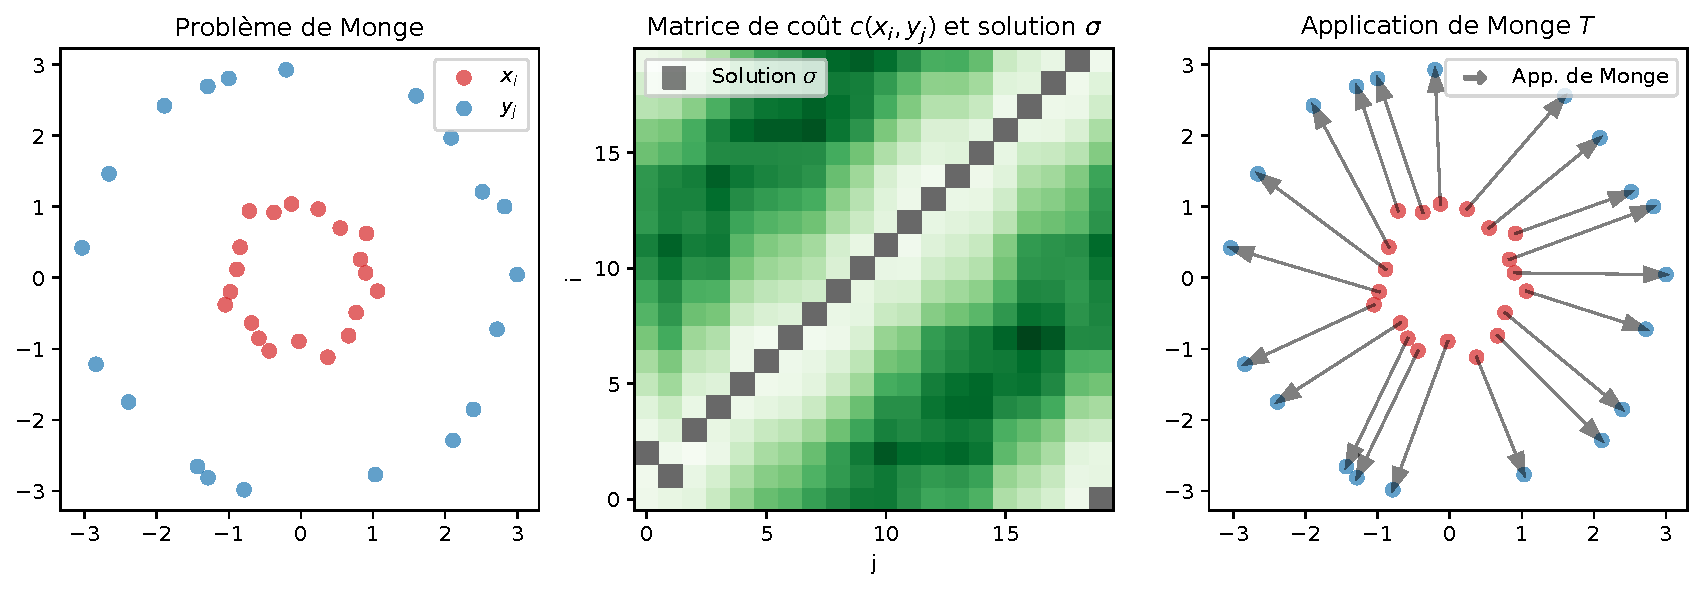
\includegraphics[width=\linewidth]{imgs/monge_example.pdf} \vspace{-10mm}
  \caption{Illustration du problème de Monge. \`A gauche les points $x_i$ et $y_j$. Au centre, la matrice de coût (la valeur du coût est proportionnelle à l'intensité de la couleur verte) pour tous les points $x_i$ et $y_j$ ordonnés par angle, et la solution optimale $\sigma$ (en gris). \`A droite, application de Monge qui résout~\eqref{eq:monge_discret}.}
  \label{fig:monge}
\end{figure}


\paragraph{Problème de Monge entre mesures de probabilité}

Le problème précédent peut s'étendre à deux mesures de probabilité $\mu$ et $\nu$ sur des ensembles $\mathcal{X}$ et $\mathcal{Y}$. On cherche une application $T:\mathcal{X} \to \mathcal{Y}$ qui envoie $\mu$ sur $\nu$ en minimisant un coût de transport de la forme
\begin{equation}
  \label{eq:monge}
 \inf_{T_\# \mu = \nu} \int c\bigl(x,T(x)\bigr)\,\mathrm{d}\mu(x),
\end{equation}
 où la notation  $T_\# \mu$ désigne la loi de la variable $T(X)$ pour $X\sim \mu$.

Lorsque les mesures sont discrètes et s'écrivent 
$\mu = \sum_{i=1}^n a_i \delta_{x_i}$ et $\nu = \sum_{j=1}^m b_j \delta_{y_j}, $
%le problème devient
% \[
%   \inf_{T_\# \mu = \nu} \sum_{i=1}^n a_i\,c\bigl(x_i,T(x_i)\bigr).
% \]
la contrainte $T_\# \mu = \nu$ se traduit par $\sum_{i=1}^n a_i \delta_{T(x_i)}
= \sum_{j=1}^m b_j \delta_{y_j}$, elle est donc très rigide. En particulier,
l'existence d'un tel $T$ n'est pas garantie : une mesure portée par un unique
point $x_0$ ne peut pas être envoyée vers une mesure portée par plusieurs points
par exemple.



\begin{figure}[t]
  \centering
  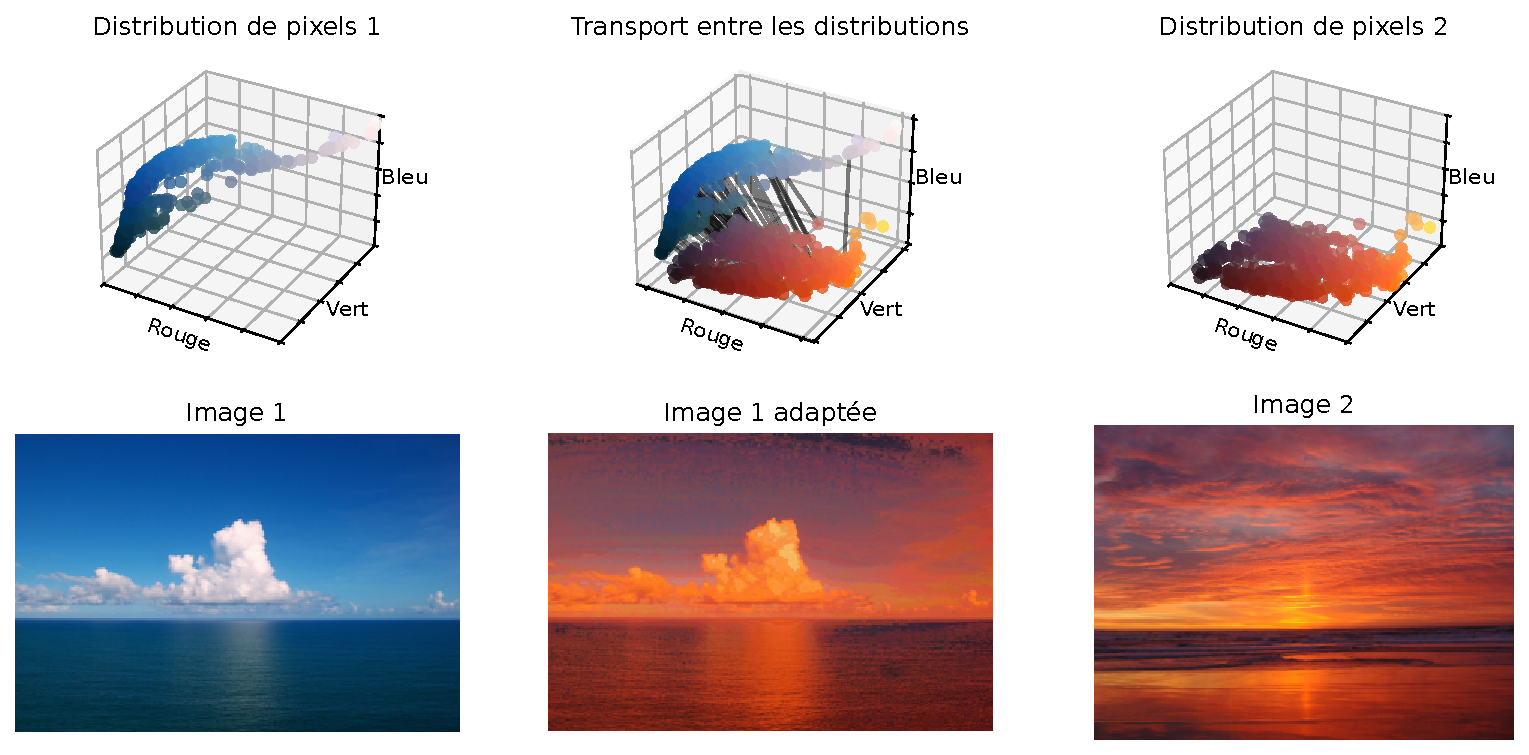
\includegraphics[width=\linewidth]{imgs/images_color_adapt.pdf} \vspace{-7mm}
  \caption{Illustration du transfert de couleur entre deux images. Les pixels de l'image source sont représentés par des points dans l'espace RGB (en haut à gauche), et les pixels de l'image cible par d'autres points (en haut à droite). Le transport optimal calcule un couplage entre ces deux ensembles de points, permettant de transférer les couleurs de l'image source vers l'image cible (milieu bas).}
  \label{fig:color_transfer}
\end{figure}

\begin{figure}[t]
  \centering
  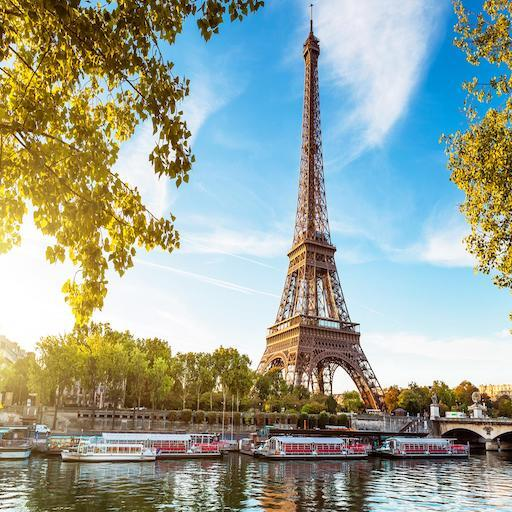
\includegraphics[width=0.3\linewidth]{imgs/eiffel.jpg} 
  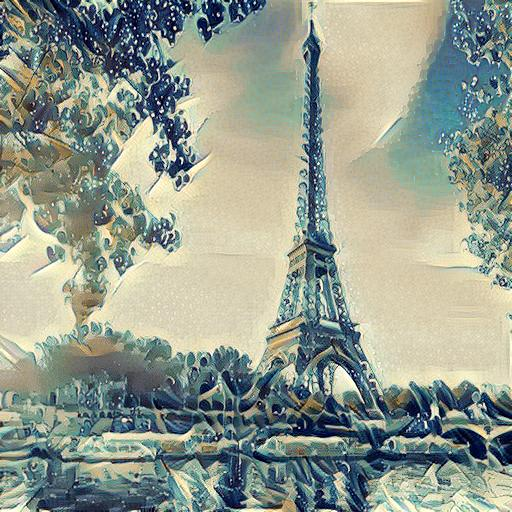
\includegraphics[width=0.3\linewidth]{imgs/eiffel_film_90.jpg} 
  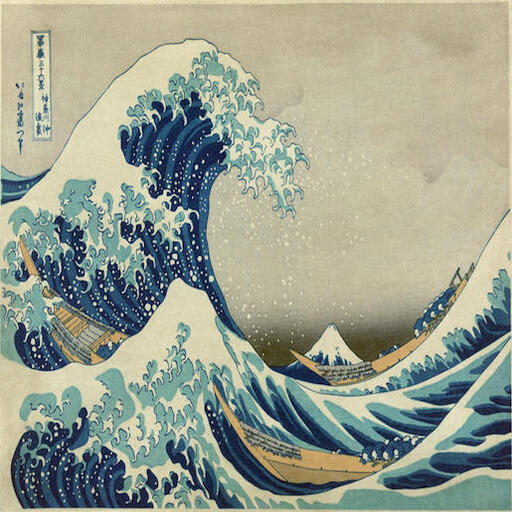
\includegraphics[width=0.3\linewidth]{imgs/hokusai.jpg} 
  \caption{Exemple de transfert de style entre deux images, extrait de~\cite{boite2025differentiable}. L'image de gauche est l'image source, l'image de droite est l'image cible. Le transport optimal est calculé entre les deux images dans un espace latent de réseau de neurones, et permet de transférer le style de l'image cible vers l'image source (image du milieu).}
  \label{fig:style_transfer}
\end{figure}

\paragraph{Application : transfert de couleur entre images}

Cette formulation suffit déjà pour construire des applications élémentaires en
image. Pour transférer les couleurs entre deux images contenant le même nombre
de pixels par exemple~\cite{dss10fast}, on représente chaque pixel de l'image
source par sa couleur $x_i$, et chaque pixel de l'image cible par sa couleur
$y_j$. L'appariement optimal associe alors à chaque couleur source une couleur
cible proche au sens du coût choisi ; on donne au pixel source $i$ la couleur
$y_{\sigma(i)}$ tout en conservant sa position spatiale, comme illustré par la Figure~\ref{fig:color_transfer}. La même idée peut être
appliquée à des descripteurs plus riches ou dans des espaces latents pour faire
du transfert de style par exemple~\cite{Mroueh:2019aa,boite2025differentiable}, comme illustré par la Figure~\ref{fig:style_transfer}.



\subsection{Transport de Kantorovich  }
\begin{figure}[ht]
  \centering
  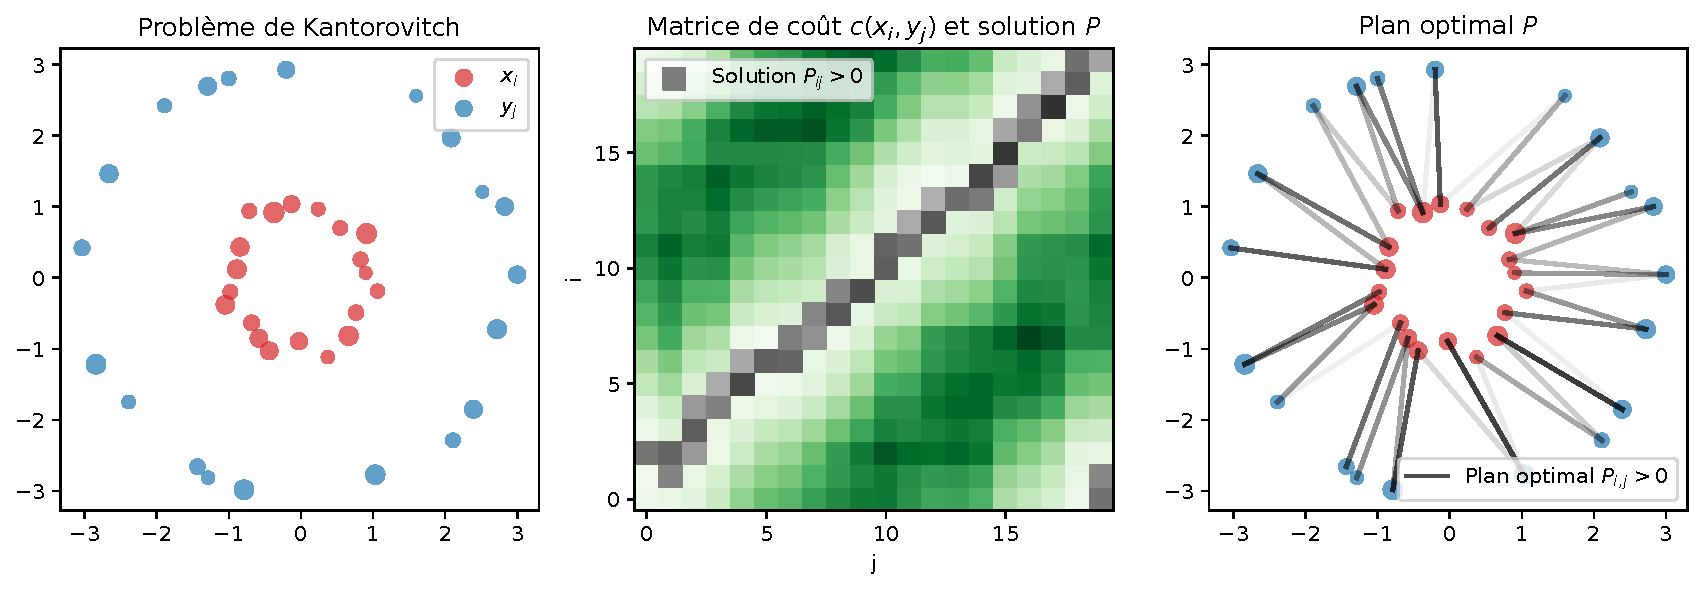
\includegraphics[width=\linewidth]{imgs/kanto_example.pdf} \vspace{-10mm}
  \caption{Illustration du problème de Kantorovich. \`A gauche, les points $x_i$ et $y_j$ avec des masses non uniformes, au centre la matrice de coûts pour tous les points $x_i$ et $y_j$ ordonnés par angle et une solution optimale $P$, à droite le plan de transport associé. L'intensité des segments est proportionnelle à la masse transportée.}
  \label{fig:kanto}
\end{figure}

Le tournant historique décisif vient des travaux de Leonid Kantorovich au milieu du XXe siècle, travaux pour lesquels il obtiendra le prix Nobel d'économie en 1975 \cite{Kantorovich1942}. A la place d'une application $T$, il cherche un couplage (appelé \emph{plan de transport}) $\pi$ entre $\mu$ et $\nu$, autrement dit une mesure de probabilité sur $\mathcal{X} \times \mathcal{Y}$ dont les marginales sont $\mu$ et $\nu$ (on note $\Pi(\mu,\nu)$ l'ensemble de ces couplages). Le plan $\pi$ indique comment la masse se répartit de $\mu$ vers $\nu$. Le problème d'optimisation posé par Kantorovich, relaxation de celui de Monge~\eqref{eq:monge},  s'écrit 
\begin{equation}
  \inf_{\pi \in \Pi(\mu,\nu)} \int c(x,y)\,\mathrm{d}\pi(x,y),
\label{eq:kanto} 
\end{equation}
Cette relaxation rend le problème convexe et donc beaucoup plus simple à étudier que celui  de Monge. En particulier, sous des hypothèses assez simples sur les espaces $\mathcal{X}$, $\mathcal{Y}$ et sur la régularité sur $c$, on peut montrer que le problème a toujours des solutions.     
 
Dans le cas de mesures discrètes $\mu = \sum_{i=1}^n a_i \delta_{x_i}$ et $\nu = \sum_{j=1}^m b_j \delta_{y_j}$, le plan $\pi$ se résume à une matrice  $P \in \mathbb{R}_+^{n\times m}$ et le problème devient
\begin{equation}
  \min_{P \in \Pi(a,b)} \sum_{i=1}^n \sum_{j=1}^m c(x_i,y_j)P_{ij}.
  \label{eq:kanto_discret}
\end{equation}
avec
\[
  \Pi(a,b)=\left\{P\in\mathbb{R}_+^{n\times m}\,;\,P\mathbf{1}_m=a,\;P^\top\mathbf{1}_n=b\right\},
\]
où $\mathbf{1}_n$ est le vecteur colonne constitué de $1$ et de longueur $n$. Pour $n$ et $m$ du même ordre de grandeur, ce
problème \eqref{eq:kanto_discret} de programmation linéaire  peut être résolu en
$O(n^3\log(n))$ par exemple par l'algorithme de \textit{network
simplex}~\cite{Ahuja1993}. Un exemple est proposé en Figure~\ref{fig:kanto} pour des points du plan et un coût quadratique.



\begin{figure}[t]
  \centering
  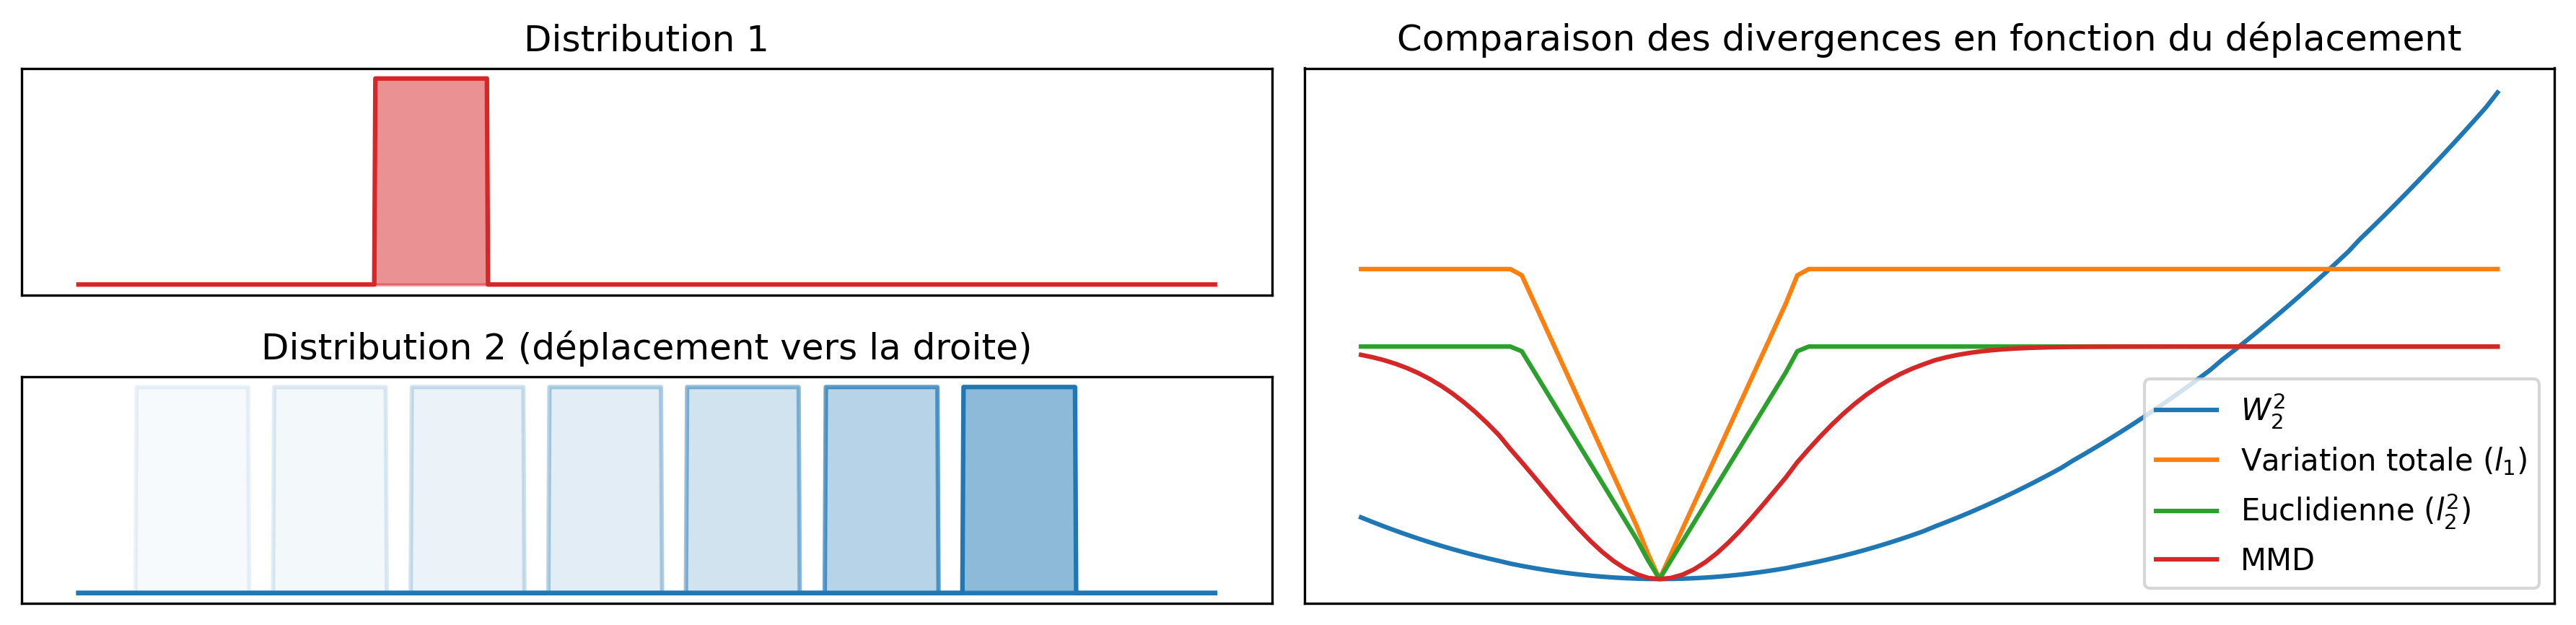
\includegraphics[width=\linewidth]{imgs/wass_plot.png} \vspace{-7mm}
  \caption{Comparaison de différentes divergences entre deux distributions en fonction du déplacement de la moyenne de la distribution cible (en bas à gauche, en bleu). Les différente divergences, la variation totale, l'euclidienne et le MMD sont comparées sur la droite à la distance de transport optimal $W_2^2$.}
  \label{fig:wass_plot}
\end{figure}


\paragraph{Distances entre mesures de probabilité}
Lorsque l'on choisit comme fonction de coût $c(x,y)=\|x-y\|^p$ sur $\mathcal{X} =\mathcal{Y} =  \mathbb{R}^d$, avec $p\geq 1$, on peut montrer que la quantité 
\[
  W_p(\mu,\nu)
  =
  \left(
  \inf_{\pi \in \Pi(\mu,\nu)}
  \int \|x-y\|^p\,\mathrm{d}\pi(x,y)
  \right)^{1/p}
\]
définit une distance sur les mesures de probabilité ayant un moment d'ordre $p$
fini, appelée souvent distance de Wasserstein ou de Monge--Kantorovich. Sur un
espace compact, cette distance métrise la convergence faible des mesures de
probabilité \cite{Villani2009}. Cette propriété qui s'étend à des cas bien plus
généraux que des espaces euclidiens est une des grandes forces du transport
optimal, qui permet de définir des distances entre mesures de probabilité sur
des espaces très généraux. {Une illustration de la valeur de la distance de
Wasserstein  par rapport à d'autres divergences est proposée en
Figure~\ref{fig:wass_plot}. Sur cet exemple, on voit que la distance de
Wasserstein peut comparer des distributions avec des support différents, n'a pas
de point stationnaire non optimal et qu'un
(sous-)gradient pertinent peut toujours être calculé. Pour ces raisons, le transport optimal est aujourd'hui beaucoup utilisé pour définir des distances en apprentissage statistique, comme on le détaille sans les sections~\ref{sec:comparer-distributions} et~\ref{sec:attache}.}


% \rf{Pour finir cette partie, signalons que le
% transport optimal est de plus en plus utilisé dans des applications
% d'apprentissage statistique, notamment pour sa capacité à comparer des
% distributions avec des support différents et le fait qu'un (sous-)gradient
% pertinent peut toujours être calculé comme illustré par la Figure
% \ref{fig:wass_plot}, où l'on voit que la distance de Wasserstein n'a pas de
% point stationnaire non optimal sur l'exemple.}
 




\begin{figure}[t]
  \centering
  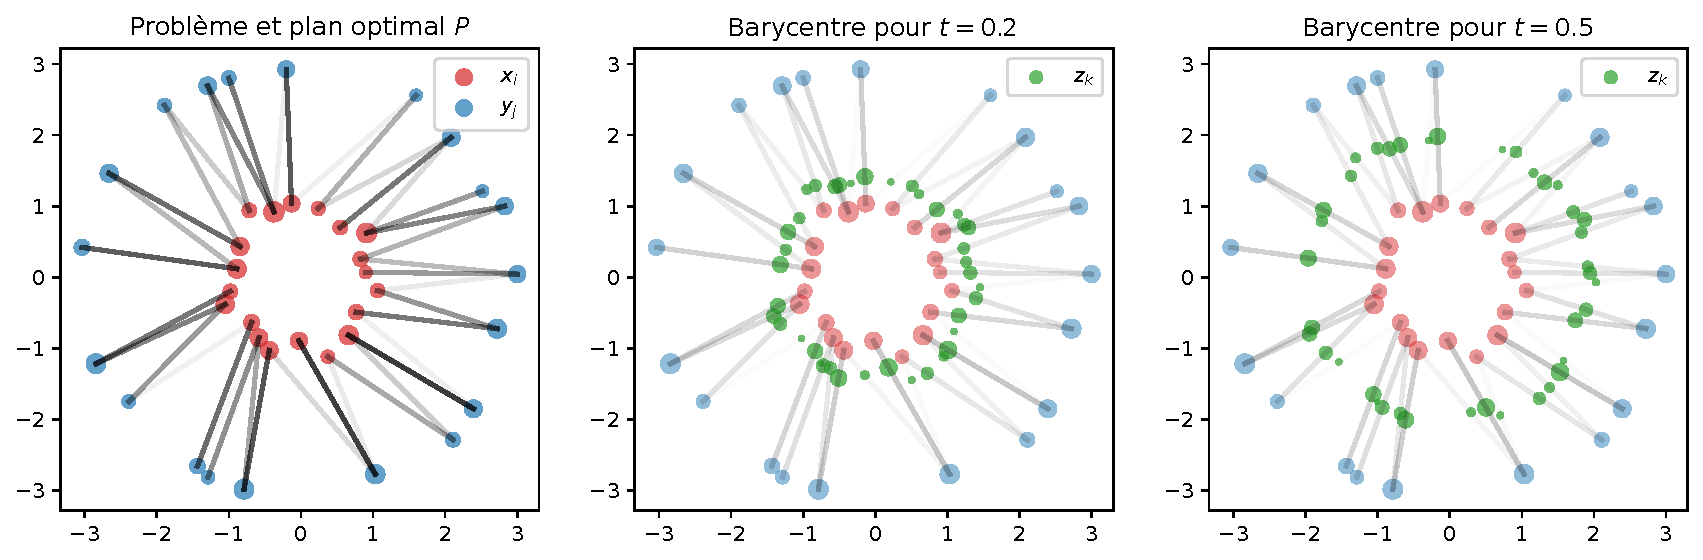
\includegraphics[width=\linewidth]{imgs/bary_example.pdf} \vspace{-5mm}
  \caption{Illustration de l'interpolation de McCann entre deux mesures de probabilité. Les mesures (en rouge et en bleu) et la solution du transport optimal sont représentées à gauche et les barycentres (en vert) pour $t=0.2$ et $t=0.5$ au milieu et à droite.}
  \label{fig:bary}
\end{figure}

\paragraph{Interpolation entre mesures}
Comme expliqué en introduction, le transport permet également de définir des interpolations géométriquement pertinentes entre mesures.
Si \(\pi\in\Pi(\mu_0,\mu_1)\) est un plan optimal pour~\eqref{eq:kanto_discret}, on peut définir pour tout \(t\in[0,1]\) 
\[ \mu_t=\psi_t\#\pi, \;\text{ où } \psi_t(x,y)=(1-t)x+ty.
\]
Le chemin \((\mu_t)_{t\in[0,1]}\) dans l'espace des mesures de probabilités est appelé l'interpolation de McCann entre \(\mu_0\) et \(\mu_1\) (voir la Figure~\ref{fig:bary} pour une illustration avec des mesures discrètes). De manière équivalente, si \((X,Y)\) a pour loi \(\pi\),
alors \(\mu_t\) est la loi de \((1-t)X+tY\). Cette interpolation peut être étendue au cas de plus de 2 mesures via la définition des barycentres de Wasserstein~\cite{carlier2010barycenter}. La section~\ref{sec:barycenters} décrit de nombreuses applications de ces interpolations en TSI, notamment en synthèse de texture.


\begin{figure}[t]
  \centering
  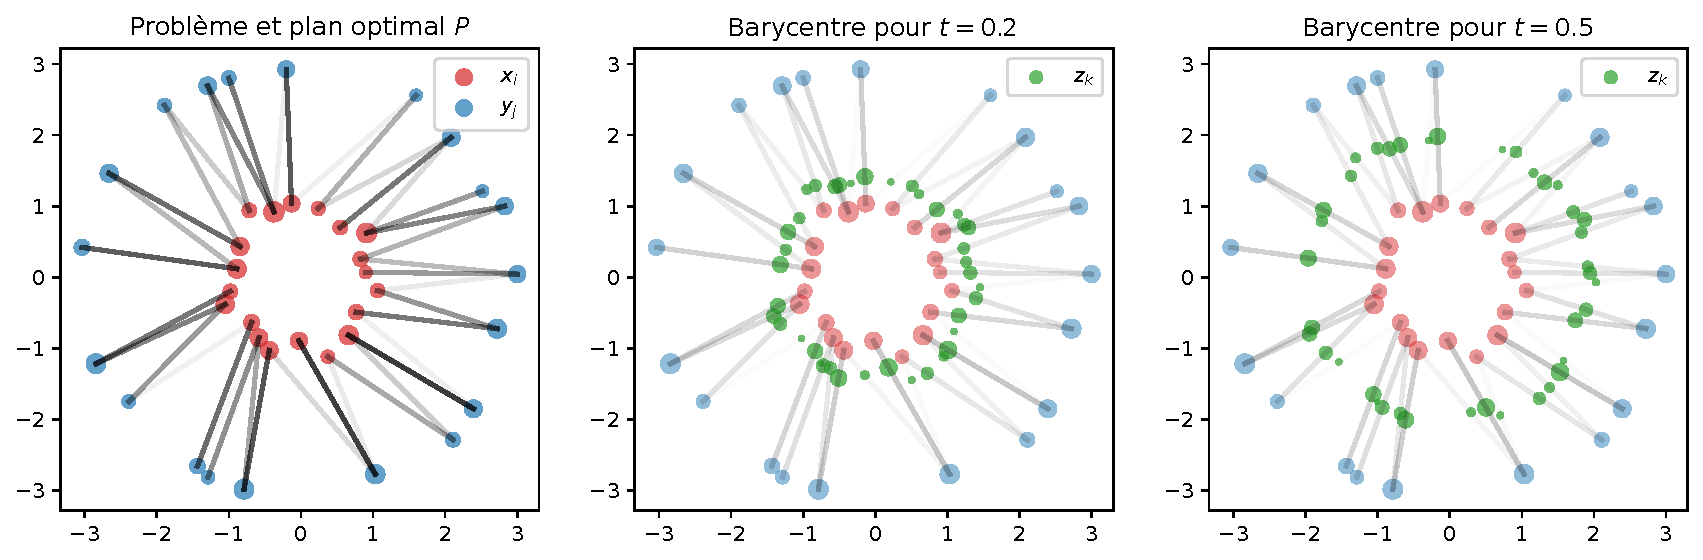
\includegraphics[width=\linewidth]{imgs/bary_example.pdf} \vspace{-5mm}
  \caption{Illustration de l'interpolation de McCann entre deux mesures de probabilité. Les mesures et la solution du transport optimal sont représentées à gauche et les barycentres pour $t=0.2$ et $t=0.5$ au milieu et à droite.}
  \label{fig:bary}
\end{figure}


\paragraph{Dualité.}
Un autre apport majeur de la formulation de Kantorovich est la dualité. Sous des hypothèses usuelles, le coût optimal peut aussi s'écrire
\[
  \sup_{\substack{\varphi(x)+\psi(y)\leq c(x,y)\\\varphi,\psi \in C_b(\R^d)}}
  \left\{
    \int \varphi\,\mathrm{d}\mu
    +
    \int \psi\,\mathrm{d}\nu
  \right\},
\] où $C_b(\R^d)$ désigne les fonctions continues bornées sur $\R^d$. 
Dans le cas $c(x,y)=\|x-y\|$, on obtient la formule de dualité de Kantorovich--Rubinstein :
\[
  W_1(\mu,\nu)
  =
  \sup_{\|f\|_{\mathrm{Lip}}\leq 1}
  \int f\,\mathrm{d}(\mu-\nu).
\]
Cette formulation duale joue un rôle central en apprentissage auomatique, comme par exemple dans les Wasserstein GAN~\cite{Arjovsky2017}.
%, car elle remplace une optimisation sur les couplages par une optimisation sur des fonctions tests.

\paragraph{Formulation dynamique}
Les distances de Wasserstein ont aussi une formulation dynamique, due à Benamou et Brenier~\cite{BenamouBrenier2000}, dans laquelle on ne cherche plus un plan de transport $\pi$ mais un chemin $(\mu_t)_{t=0}^1$ entre $\mu_0$ et $\mu_1$ et un champ de vitesse $v_t$ dont le flot génère cette interpolation. 
Cette formulation dynmique s'écrit
\begin{equation}
  W_p^p(\mu_0,\mu_1)
  =
  \inf_{\substack{(\mu_t,v_t)~\sim (CE)\\ \mu_{t=0}=\mu_0,\quad \mu_{t=1}=\mu_1}}
  \int_0^1 \int_{\mathbb{R}^d}
  \|v_t(x)\|^p d\mu_t(x)\,\mathrm{d}t,
  \label{eq:dyn}
\end{equation}
où la contrainte $(\mu_t,v_t)~\sim (CE)$ signifie que $(\mu_t,v_t)$ satisfont l'équation suivante (dite équation de continuité, ou de conservation de la masse) au sens des distributions
\[\partial_t \mu_t + \nabla\!\cdot(\mu_t v_t)=0.\]
Cette interprétation révèle les liens forts entre le transport optimal et les modèles génératifs fonctionnant par discrétisation d'équations différentielles (stochastiques ou non), comme les modèles de diffusion ou le {\em Flow Matching}. Elle aide notamment à comprendre dans quels cas ces modèles coïncident ou pas avec le transport optimal (voir la section~\ref{sec:generatif}). 

%\section{Du transport optimal computationnel au TSI}

\section{Le tournant du transport optimal computationnel}

\paragraph{Des débuts timides}
Alors que la recherche mathématique autour du transport optimal est foisonnante dans les années 1990, notamment avec des écoles françaises et italiennes très dynamiques, l'utilisation pour les applications en TSI reste timide. 
L'une des premières apparitions du transport optimal dans le domaine est l'introduction de l'\emph{Earth Mover's Distance} (EMD) en vision par ordinateur au début des années 2000, utilisée pour comparer des histogrammes de caractéristiques, typiquement pour des applications en recherche d'images ou en appariement de descripteurs \cite{Rubner2000}. Lorsque les histogrammes ont même masse totale et que le coût au sol est une distance, cette quantité coïncide avec $W_1$. Le transport est aussi utilisé pour la comparaison de caractéristiques locales pour la mise en correspondance d'image~\cite{rabin2009statistical}. Le succès du transport dans ces applications vient de son bon comportement vis-à-vis des translations, petites déformations ou erreurs de localisation. 
%Remarquons en effet que pour deux masses de Dirac, $  W_1(\delta_{x_0},\delta_{x_1}) = |x_0-x_1|.$
%Deux images peuvent avoir des distributions de caractéristiques proches tout en présentant un léger décalage des masses entre bins voisins : une distance de transport est alors plus pertinente qu'une comparaison bin à bin. 

Le manque d'algorithmes réellement efficaces pour calculer des solutions numériques du transport reste cependant longtemps un frein non négligeable à son adoption plus large. Les algorithmes exacts sont en effet trop coûteux pour les problèmes apparaissant en imagerie, où $n$ et $m$ sont souvent gigantesques. Seuls des problèmes spécifiques peuvent être traités efficacement, lorsque des solutions explicites du transport optimal peuvent être obtenues, comme dans le cas unidimensionnel ou le cas des distributions gaussiennes. %Cela couvre par exemple l'égalisation ou le transfert d'histogrammes de niveaux de gris, la comparaison de signatures spectrales unidimensionnelles, ou certains modèles statistiques gaussiens.


\paragraph{Montée en puissance}
Le début des années 2010 constitue un tournant majeur pour le transport optimal computationnel, avec l'introduction en quelques années de plusieurs algorithmes efficaces de calcul de solutions approchées du problème. Un exemple saillant en 2013 est la régularisation entropique proposée par Marco Cuturi, qui consiste à régulariser~\eqref{eq:kanto_discret} en lui ajoutant un terme d'entropie pour le rendre strictement convexe \cite{Cuturi2013}
\[
  \min_{P \in \Pi(a,b)}
  \sum_{i=1}^n \sum_{j=1}^m c(x_i,y_j)P_{ij}
  +
  \varepsilon
  \sum_{i=1}^n\sum_{j=1}^m
  P_{ij}\bigl(\log P_{ij}-1\bigr).
\]
Les solutions de ce transport régularisé sont plus faciles à estimer, notamment
grâce à l'algorithme de Sinkhorn~\cite{SinkhornKnopp1967} et peuvent exploiter le calcul parallèle sur GPU. La
Figure~\ref{fig:label} illustre l'effet de cette régularisation entropique sur
les solutions du transport optimal. 

\begin{figure}[ht]
  \centering
  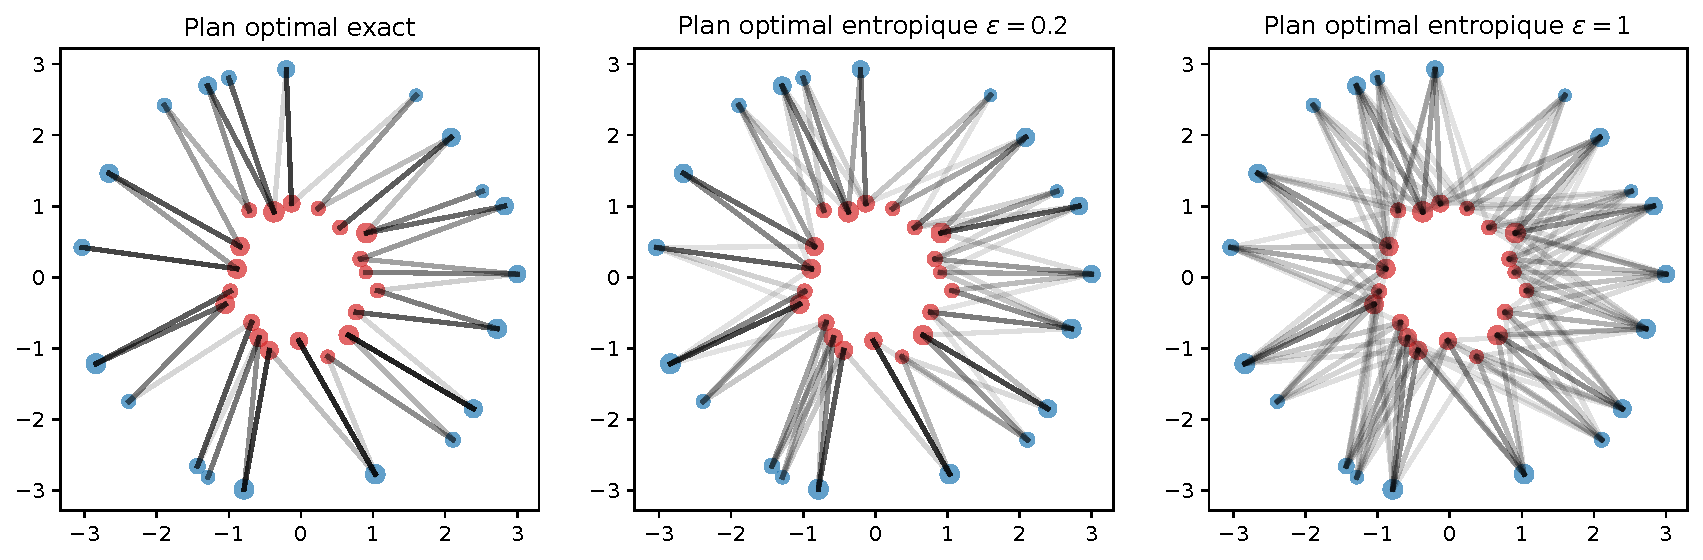
\includegraphics[width=\linewidth]{imgs/entropic_example.pdf} \vspace{-10mm}
  \caption{Illustration de l'effet de la régularisation entropique sur le transport optimal. La régularisation entropique rend le plan de transport plus diffus, ce qui peut être utile pour certaines applications en TSI.}
  \label{fig:label}
\end{figure}

D'autres algorithmes approchés ou spécialisés sont proposés à la même période,
comme les méthodes semi-discrètes, où l'une des mesures est continue et l'autre
discrète \cite{Merigot2011}, ou les approches dites par \og tranches \fg,
introduites dans~\cite{Rabin2012,bonneel2015sliced} pour calculer des
barycentres de textures. Certaines approches sont spécialisées pour des espaces
spécifiques (comme le cercle, voir~\cite{dss10fast}) ou des mesures
particulières : la distance $W_2$ entre gaussiennes par exemple a une formule
close~\cite{dowson1982frechet} et une version du transport optimal adaptée aux
mélanges de gaussiennes est proposée
dans~\cite{delon2020wasserstein,boite2025differentiable}. 

On peut aussi citer les méthodes de résolution du transport optimal à l'aide de réseaux de neurones, qui permettent de traiter des mesures de probabilité continues dans des espaces de grande dimension~\cite{seguy2018large,makkuva2020optimal,korotin2022neural}. Des approches spécifiques sont également développées pour calculer rapidement des  barycentres de Wasserstein approchés~\cite{cuturi2014fast,benamou2015iterative,tanguy2024computing}, problème notoirement difficile.
Le développement de ces algorithmes de calcul efficaces change la donne : le transport optimal s'impose progressivement comme un outil central  pour comparer ou interpoler des distributions en TSI et en apprentissage machine.

%\rf{RF: j'ajouterai un paragraphe sur les cas particuliers (D, cercle,gaussienne et mixture?}


\section{Applications variées en TSI}

Passons en revue quelques applications du transport optimal en TSI, en insistant sur les aspects qui le rendent particulièrement adapté à ce domaine. Avant tout, remarquons que le transport optimal ne s’applique pas directement à une image ou à un signal : il faut d’abord choisir ce qui joue le rôle de masse (pixels, couleurs, fréquences, patchs, caractéristiques apprises, réponses de certaines couches d'un réseau de neurones) ainsi que le coût associé au déplacement de cette masse. Ce choix de représentation est déterminant.


\subsection{Comparer des distributions}
\label{sec:comparer-distributions}
Un des rôles centraux du transport optimal en TSI est de comparer des
distributions en tenant compte de leur géométrie, ce qui prolonge directement
l'usage de l'EMD pour la recherche d'images~\cite{Rubner2000}. Il est utilisé
pour comparer des histogrammes de couleurs ou de textures~\cite{Rabin2012}, des
spectres ou des
spectrogrammes~\cite{flamary2016optimal,cazelles2020wasserstein}, des
distributions sur variétés~\cite{Solomon2015}, des ensembles de descripteurs
locaux~\cite{rabin2009statistical}, ou encore des sorties de modèles génératifs
\cite{Arjovsky2017}. Il est notable que l’un des indicateurs de performance les plus utilisés pour les modèles génératifs d'images, la "Fréchet inception distance" ou FID, repose sur une distance de
Wasserstein entre des distributions gaussiennes \cite{heusel2017gans} dans un
espace de représentation appris par un réseau de type {\em Inception}. 



\subsection{Aligner et transporter des distributions} Un des aspects les plus
puissants du transport optimal est qu'en plus de mesurer la distance entre deux
distributions, il fournit un couplage optimal entre elles. Ce couplage peut être
utilisé pour aligner ou transporter des distributions, ce qui est utile dans de
nombreuses applications. Des applications en TSI sont par exemple le recalage
d'images~\cite{Haker2004}, le recalage de formes~\cite{feydy2017optimal}, le
recalage de nuages de points~\cite{bonneel2019spot}, le transfert de
couleurs~\cite{Ferradans2014} ou de style~\cite{Mroueh:2019aa,boite2025differentiable}.

% CITER \cite{Haker2004} pour le recalage d'image ?

Le couplage optimal peut aussi servir à transporter des masses entre
distributions et donc à adapter des données. Ceci est particulièrement utile en apprentissage statistique, par
exemple en adaptation de domaine, où l'on cherche à transférer un modèle appris
sur une distribution source vers une distribution cible différente mais proche
\cite{Courty2017}. Ce genre d'approche a également été étendu au cas
multi-domaines \cite{turrisi2022multi,montesuma2021wasserstein} ou avec des approximations gaussiennes pour
normaliser des signaux biomédicaux \cite{gnassounou2023convolutional,gnassounou2026psdnorm}.

 %: les histogrammes ne sont plus comparés bin par bin, mais à travers le coût de déplacement entre leurs bins. Le même principe 


% Il sert aussi en adaptation de domaine : on aligne une distribution source et
% une distribution cible dans un espace de caractéristiques, tout en conservant
% une contrainte statistique ou de classe \cite{Courty2017}. 
\subsection{Aligner des distributions sur des graphes}{Le transport optimal a
également été étendu pour aligner des données définies par des relations paires à paires entre les points, comme des graphes \cite{Memoli2011,Solomon2015}. 
Ces distances, dites de Gromov-Wasserstein, modélisent des signaux sur graphes
comme des distributions et permettent de comparer des
graphes  de taille différentes et de trouver des alignements entre leurs noeuds \cite{Solomon2015,vayer2019optimal}.
Des applications de ces distances ont été proposées
pour aligner} des graphes d'interactions multi-omiques entre cellules
\cite{demetci2022scot}, pour l'alignement de signaux d'activation du cerveau
\cite{thual2022aligning}, ou encore pour l'alignement entre langages
\cite{alvarez2018gromov}.


\subsection{Servir d'attache aux données}
\label{sec:attache}
Le transport optimal sert également d'attache aux données dans des problèmes inverses, notamment lorsque l'erreur entre observation et simulation relève moins d'un bruit additif que d'un décalage ou d'une redistribution de masse. Par exemple, les auteurs de~\cite{Delbracio:2020aa} l'utilisent sur les caractéristiques d'un réseau de type VGG pour mesurer la similarité perceptuelle entre deux images et l'intégrer dans une fonction de perte. Le transport est utilisé dans~\cite{Adrai:2023aa} pour améliorer la qualité perceptuelle de n'importe quel modèle de restauration entraîné pour minimiser une erreur quadratique moyenne. Des distances de transport sont aussi utilisées en imagerie sismique pour réduire la sensibilité de l'inversion de formes d'onde aux minima locaux liés aux décalages de phase \cite{Metivier2016}. 
Lorsque les masses ne doivent pas être conservées exactement, par exemple à
cause d'occultations ou de variations d'intensité, les variantes non équilibrées
du transport optimal pénalisent la création ou la destruction de masse sans
l'interdire \cite{Chizat2018}.
Le transport optimal a aussi été utilisé en segmentation d'image : chaque région de l’image peut être représentée par une distribution de caractéristiques. Une distance de Wasserstein mesure alors son accord avec un modèle de région, tout en tolérant de petites variations dans les caractéristiques observées~\cite{peyre2012wasserstein,papadakis2017convex}.

Enfin, il peut définir une perte lorsque les sorties ont une géométrie naturelle, par
exemple dans des problèmes de prédiction multi-étiquettes \cite{Frogner2015} ou
de prédiction structurée \cite{brogat2022learning}. Il est aussi utilisé pour
apprendre des dictionnaires de représentation de
données~\cite{sandler2011nonnegative,schmitz2018wasserstein}. 



\subsection{Interpoler, synthétiser}
\label{sec:barycenters}
Le transport optimal définit des géodésiques et des barycentres entre distributions, qui respectent la géométrie de ces dernières. En TSI, ces barycentres ont beaucoup été explorés pour interpoler des textures, au départ en utilisant des représentations à l'aide de filtres multi-échelles orientés~\cite{Rabin2012}, puis des modèles de textures gaussiennes~\cite{Xia2014}, et plus récemment des distributions elliptiques sur les activations d'un réseau convolutionnel~\cite{Vacher2020} (voir la Figure \ref{fig:interpolation_texture}). Les barycentres de Wasserstein ont été étendus pour interpoler des données variées, comme des formes, des images de réflectances ou des distributions de couleur~\cite{Solomon2015}.

Le transport optimal est également utilisé pour la synthèse de texture à partir d'un exemple~\cite{Galerne2018,leclaire2022gretsi,Heitz:2020aa,Houdard2023}. Dans ces approches, le transport  est utilisé soit comme une fonction de perte, soit comme un outil permettant de transférer des caractéristiques d'une texture vers une autre, ces caractéristiques étant souvent des distributions de patchs ou de réponses de réseaux de neurones. %optimisés pour la reconnaissance d'objets.





\begin{figure}[t]
  \centering
  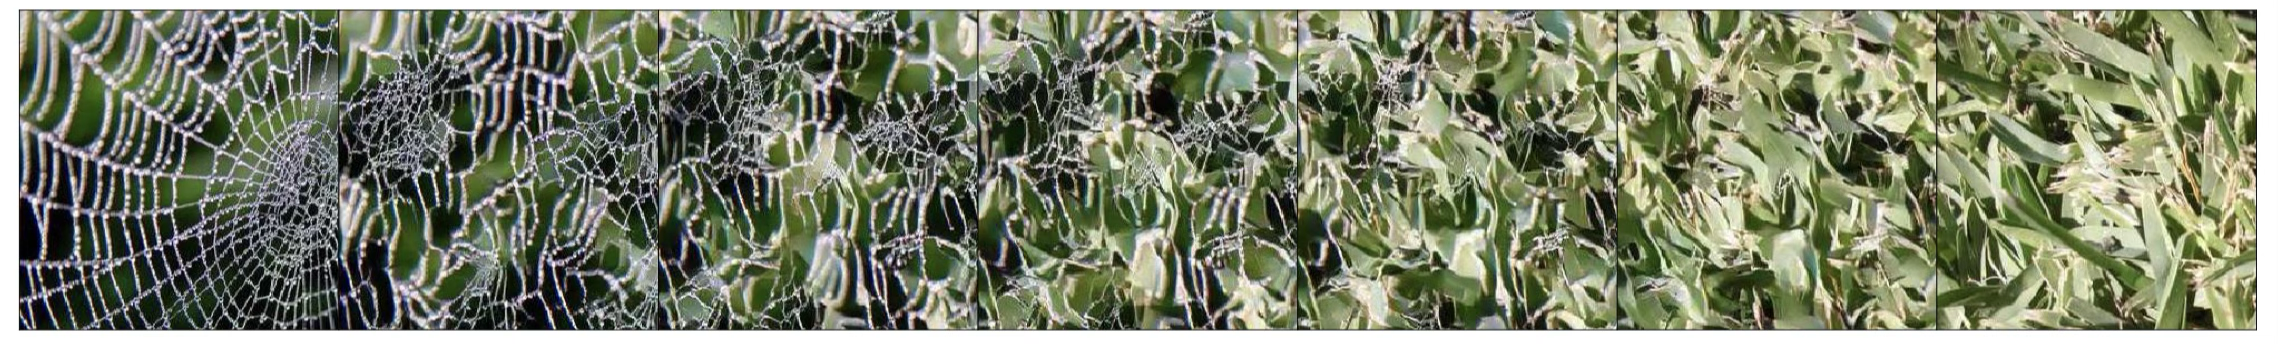
\includegraphics[width=\linewidth]{imgs/interpolation_texture_vacher.png} \vspace{-5mm}
  \caption{Exemple d'interpolation de textures utilisant l'approche~\cite{Vacher2020}, les textures sont représentées dans un espace latent de réseau de neurones par des modèles Gaussiens, dont on peut calculer explicitement les barycentres. Les images à gauche et à droite sont les textures de départ, et les images intermédiaires sont des interpolations cohérentes entre ces deux textures.}
  \label{fig:interpolation_texture}
\end{figure}




\subsection{Générer des données et comprendre des modèles génératifs}
\label{sec:generatif}
Plus généralement, le transport optimal est devenu un ingrédient central de nombreux modèles d'apprentissage. Il peut aussi servir à comparer des mesures empiriques plutôt que des vecteurs fixes, ce qui explique son usage en adaptation de domaine, en apprentissage sur ensembles de points ou en génération. Les Wasserstein GAN ont ainsi popularisé l'usage de la forme duale de $W_1$ comme critère d'entraînement de modèles génératifs \cite{Arjovsky2017}. 

Les liens avec les modèles génératifs basés sur des flots sont également importants. Les modèles de diffusion et les modèles de type \emph{Flow Matching} apprennent des chemins, stochastiques ou déterministes, entre une loi simple et la loi des données~\cite{Ho2020,Song2021,Lipman2023}, en intégrant un champ de vitesse. Ces champs de vitesse vérifient l'équation de continuité (ou sa version aléatoire, l'équation de Fokker-Planck) avec l'interpolation $(\mu_t)$ qu'ils génèrent. Ils sont très proches en ce sens de la formulation dynamique de Benamou--Brenier~\cite{BenamouBrenier2000}, même si les chemins appris par ces modèles ne minimisent pas d'énergie cinétique et ne correspondent donc en général pas à du transport optimal~\cite{Hertrich2025,Pierret2026}. 

Les ponts de Schrödinger ont également été utilisés pour des applications de génération de données~\cite{DeBortoli2021} et établissent un lien plus direct entre modèles de diffusion et transport régularisé : ils cherchent à résoudre un problème de transport dynamique (donc à minimiser l'énergie~\ref{eq:dyn}) entre deux distributions, tout en tenant compte d’une diffusion aléatoire (mathématiquement, la contrainte n'est plus l'équation de continuité mais l'équation de Fokker-Planck). %Ils peuvent ainsi être vus comme une forme de transport optimal régularisé par du bruit et ont également été utilisés pour des applications de génération de données~\cite{DeBortoli2021}. %Cette perspective a notamment été utilisée pour généraliser les modèles fondés sur le score par des ponts de Schrödinger appris \cite{DeBortoli2021}. 

Sur un thème proche, les outils du transport optimal servent aussi à mieux comprendre la dynamique interne des réseaux de type
{\em transformers} : une séquence de tokens peut être vue comme une mesure empirique, et les couches successives et mécanisme d'attention du {\em transformer} modifient cette mesure, dont on peut étudier l'évolution dans le réseau afin de mieux comprendre certains comportements du modèle~\cite{Castin2025Transformers,Peyre2025OTML}.

%%% rectified flow
%ransports optimaux. Les variantes de type \emph{rectified flow} cherchent à rendre les trajectoires plus droites, donc plus faciles à intégrer numériquement \cite{Liu2023}; des travaux récents précisent cependant que cette rectification ne suffit pas, sans hypothèses supplémentaires, à calculer une application de transport optimal \cite{Hertrich2025,Pierret2026}. 

%%% mini-batch 
%En pratique, plusieurs méthodes utilisent un transport optimal calculé sur mini-batchs pour construire, à l'échelle d'un lot, des couplages plus informatifs que l'appariement indépendant et améliorer le \emph{flow matching} \cite{Pooladian2023,Tong2024}; ce substitut est efficace, mais il introduit un biais dont l'analyse commence seulement à être bien comprise \cite{Boite2026}.

\section*{Conclusion}

Ces exemples témoignent de la richesse et de la remarquable diversité des applications du transport optimal en TSI, depuis la comparaison et l’alignement des données jusqu’à leur interpolation et leur génération. Ce cadre offre ainsi un langage commun particulièrement fécond, à condition de garder à l’esprit que son efficacité dépend fortement de la représentation des données, du coût choisi et des approximations nécessaires pour rendre les calculs abordables.

\bibliographystyle{plain}
\bibliography{transport_optimal_tsi}

\end{document}
